\documentclass[12pt,]{article}
\usepackage[T1]{fontenc}
\usepackage{lmodern}
\usepackage{amssymb,amsmath}
\usepackage{ifxetex,ifluatex}
\usepackage{fixltx2e} % provides \textsubscript
% use upquote if available, for straight quotes in verbatim environments
\IfFileExists{upquote.sty}{\usepackage{upquote}}{}
\ifnum 0\ifxetex 1\fi\ifluatex 1\fi=0 % if pdftex
  \usepackage[utf8]{inputenc}
\else % if luatex or xelatex
  \ifxetex
    \usepackage{mathspec}
    \usepackage{xltxtra,xunicode}
  \else
    \usepackage{fontspec}
  \fi
  \defaultfontfeatures{Mapping=tex-text,Scale=MatchLowercase}
  \newcommand{\euro}{€}
\fi
% use microtype if available
\IfFileExists{microtype.sty}{\usepackage{microtype}}{}
\usepackage[margin=1in]{geometry}
\usepackage{graphicx}
% Redefine \includegraphics so that, unless explicit options are
% given, the image width will not exceed the width of the page.
% Images get their normal width if they fit onto the page, but
% are scaled down if they would overflow the margins.
\makeatletter
\def\ScaleIfNeeded{%
  \ifdim\Gin@nat@width>\linewidth
    \linewidth
  \else
    \Gin@nat@width
  \fi
}
\makeatother
\let\Oldincludegraphics\includegraphics
{%
 \catcode`\@=11\relax%
 \gdef\includegraphics{\@ifnextchar[{\Oldincludegraphics}{\Oldincludegraphics[width=\ScaleIfNeeded]}}%
}%
\ifxetex
  \usepackage[setpagesize=false, % page size defined by xetex
              unicode=false, % unicode breaks when used with xetex
              xetex]{hyperref}
\else
  \usepackage[unicode=true]{hyperref}
\fi
\hypersetup{breaklinks=true,
            bookmarks=true,
            pdfauthor={},
            pdftitle={},
            colorlinks=true,
            citecolor=blue,
            urlcolor=blue,
            linkcolor=magenta,
            pdfborder={0 0 0}}
\urlstyle{same}  % don't use monospace font for urls
\setlength{\parindent}{0pt}
\setlength{\parskip}{6pt plus 2pt minus 1pt}
\setlength{\emergencystretch}{3em}  % prevent overfull lines
\setcounter{secnumdepth}{0}

\author{}
\date{}
\usepackage{lineno}
\linenumbers
\usepackage{setspace}

\begin{document}

\normalsize


\renewcommand\thefigure{D\arabic{figure}} 



\section{Appendix D: Model forecasts without parameter
uncertainty}\label{appendix-d-model-forecasts-without-parameter-uncertainty}

In the main text we show results from model forecasts where we included
full model and parameter uncertainty (Fig. 6). However, the typical
approach in ecology is to use point estimates of model parameters and
only include model error. For example, to predict population size
\emph{N} at time \emph{t+1} one could do the following:

\begin{align}
\mu_{t+1} &= f(N_{t}) \\
N_{t+1} &\sim \text{Normal}(\mu_{t+1}, \sigma^2)
\end{align}

where $f(N_t)$ is some determinstic process (e.g., a linear regression
model) and $\sigma^2$ is the model error. Simulating populations in such
a way ignores variation in the parameters of $f(N_t)$. When we take this
approach to making forecasts of equilibrium cover under 1\% climate
perturbations the IPM and QBM make opposing predictions if we simply
look at the mean projection (Fig. D1). For both models, precision is
also artificially high (Fig. D2 and D3), since we know that parameter
uncertainty reduces forecast precision considerably (Fig. 6 in the main
text). All three presentations of model results (mean projection, mean
projection with model error, and forecasts with full uncertainty) can be
found in the literature, which is why we present them here as well.
However, as we state in the main text, true forecasts should only be
presented as we did in Fig. 6 of the main text.

\begin{figure}[htbp]
\centering
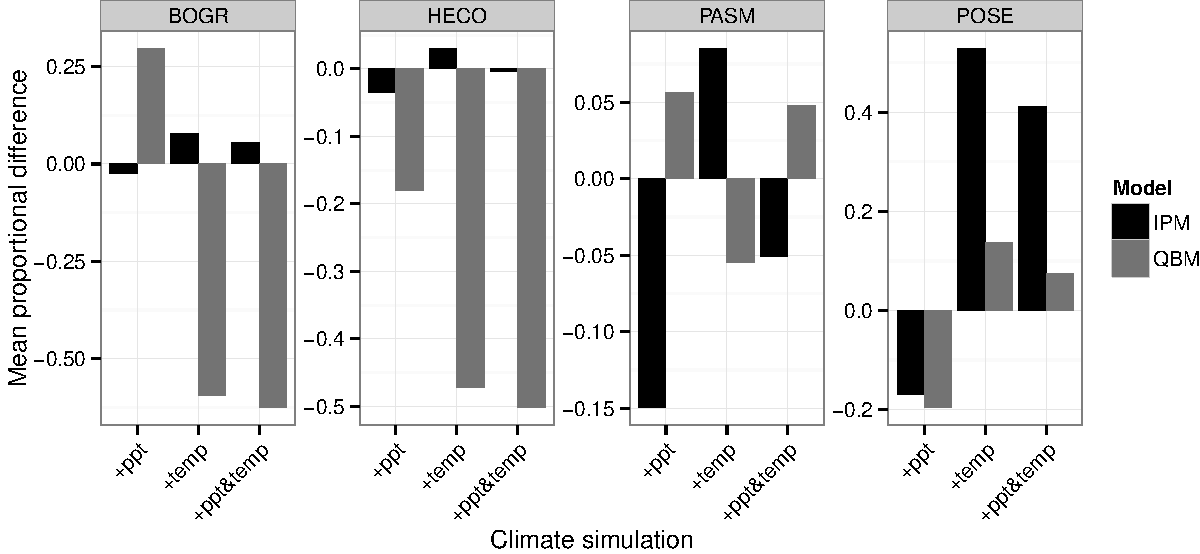
\includegraphics{appD/figure/appD-figure_d1.pdf}
\caption{Projected proportional changes in equilibrium cover caused by a
1\% increase in observed precipitation (+ppt), temperature (+temp), or
both (+ppt\&temp) as predicted by the individual-level IPM and the
population-level QBM using mean parameter values.}
\end{figure}

\begin{figure}[htbp]
\centering
\includegraphics{appD/figure/appD-figure_d2.pdf}
\caption{Projected mean (points) proportional changes in equilibrium
cover and associated 90\% quantiles (errorbars) caused by a 1\% increase
in observed precipitation (+ppt), temperature (+temp), or both
(+ppt\&temp) as predicted by the individual-level IPM using mean
parameter values. Dashed line indicates proportional change of 0.}
\end{figure}

\begin{figure}[htbp]
\centering
\includegraphics{appD/figure/appD-figure_d3.pdf}
\caption{Projected mean (points) proportional changes in equilibrium
cover and associated 90\% quantiles (errorbars) caused by a 1\% increase
in observed precipitation (+ppt), temperature (+temp), or both
(+ppt\&temp) as predicted by the population-level QBM using mean
parameter values. Dashed line indicates proportional change of 0.}
\end{figure}

\end{document}
